\chapter{Results}
Using the algorithm described above one is able to produce a NURBS representation of a structure, that has been optimized with respect to predefined boundary conditions. Examples of initial boundary conditions as well as the resulting optimized structures are presented in \autoref{sec:tests}. Additionally the described topology optimization tool enables a less complicated design workflow from the user's point of view. That workflow is described in \autoref{sec:uex}.
\section{Test Cases}
\label{sec:tests}
\todourgent[inline,author=Benni]{Put test cases here, initial condition -> resulting topology, including material saved!}
\begin{figure}[H]
\begin{center}
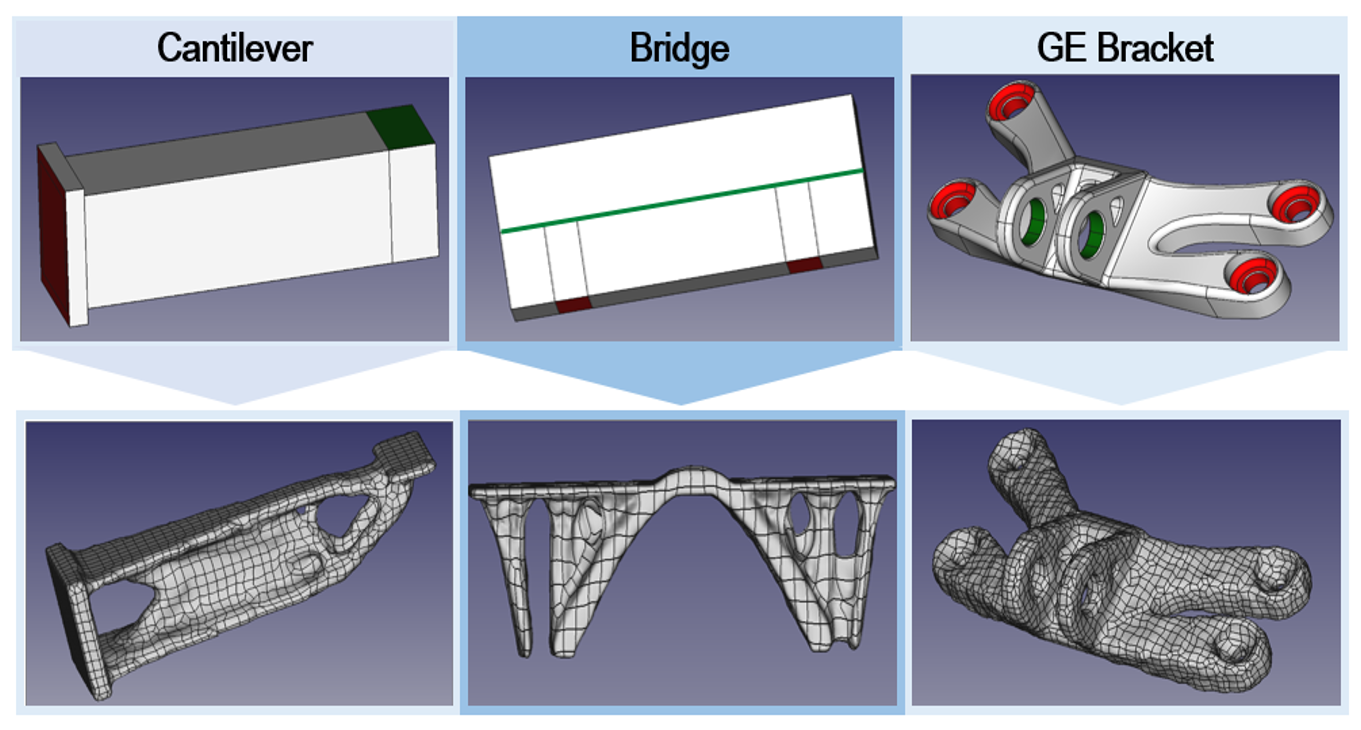
\includegraphics[width = \textwidth]{Pictures/TestCases.png}
\end{center}
\end{figure}
\todointernal[inline,author=Benni]{don't forget to cite GE Bracket!}

\section{User Experience}
\label{sec:uex}
\todourgent[inline, author=Benni]{Summarize the the resulting benefits from a user perspective. Put GUI interaction and user documentation here.}